\chapter{Example Systems} \label{ch:ExampleSystems}
this chapter is all about the actual examples that we've worked through and got an answer for.
It will tie together the VectorEqns and QG chapters and display how we are using the theory to solve problems that might represent physical wave-guides.

\section{Preliminaries}
We should recall the necessary things, such as the definition of the M-matrix, how QG problems work, that now our edges need to be directed as do our derivatives (MB I've used that derivatives INTO the vertex are positive but the opposite convention amounts to multiplying the M-matrix by -1), the vector QG system we are solving, how to build the M-matrix etc.
Also in here should be the general result for the M-matrix column contributions - similar in ilk to EKK paper which should be referenced (again here, if necessary).

Here are the curl-curl edge equations without the tildes because that'll of been explained away, and without $u_2$ because we've gotten rid of that by substitution and so can just focus on the $u_3$ and finding $\omega$. 
They're just here so that all my internal referencing will work as I write the other parts of the section!
\begin{align} \label{eq:QGEquation}
	0 &= -\bracs{\diff{}{t} + i\qm_{jk}}^2 u_{3,jk} + \bracs{\wavenumber^2 - \omega^2}u_{3,jk}.
\end{align}
\begin{subequations} \label{eq:QGVertexConditions}
	\begin{align}
		u_3 &\text{ is continuous at each } v_j\in V, \\
		0 &= \sum_{j\sim k} \bracs{\diff{}{t} + i\qm_{jk}}u_{3,jk}\bracs{v_j}.
	\end{align}
\end{subequations}

Here is the GS to \eqref{eq:QGEquation} without any boundary conditions (nb set $\eta = \bracs{\omega^2-\wavenumber^2}^{1/2}$).
\begin{align*}
	u_{3,jk} &= e^{-i\qm_{jk}t}\bracs{ C_{+}^{(jk)}e^{-i\eta t} + C_{-}^{(jk)}e^{i\eta t} }
\end{align*}

\begin{prop}[$M$-matrix entries]
	Let $\graph=\bracs{V,E}$ be an embedded graph on which the problem \eqref{eq:QGEquation}-\eqref{eq:QGVertexConditions} is posed.
	Set $\eta = \bracs{\omega^2-\wavenumber^2}^{1/2}$, and for each $I_{jk}\in E$ let $\qm_{jk} = \bracs{R_{jk}\qm}_2$ and $l_{jk} = \abs{I_{jk}}$.
	Suppose that $\dmap u = e_k$ where $e_k$ is the $k$\textsuperscript{th} canonical unit vector in $\reals^{\abs{V}}$.
	Then the $j$\textsuperscript{th} entry of $\nmap u$, and hence the $jk$\textsuperscript{th} entry in the $M$-matrix, is given by \tstk{sim symbol! also all this notation needs to be set out at some point because I don't want to write out what it all is in the proposition hypothesis like i currently have}
	\begin{align*}
		\bracs{\nmap u}_j &= 
		\begin{cases}
			\!\begin{aligned}
				0	
			\end{aligned}			
			& j \not\sim k, \\
			\!\begin{aligned}
				-\sum_{\substack{j\sim k, \\ j \text{ left}}} \eta e^{i\qm_{jk}l_{jk}} \csc\bracs{l_{jk}\eta} 
				\\ \quad - \sum_{\substack{j\sim k, \\ j \text{ right}}} \eta e^{i\qm_{kj}l_{kj}} \csc\bracs{l_{kj}\eta}
			\end{aligned}
			& j\neq k, \ j\sim k, \\
			\!\begin{aligned}
				\sum_{\substack{j\sim l, \\ j \text{ left}}} \eta\cot\bracs{l_{jl}\eta}
				+ \sum_{\substack{j\sim l, \\ j \text{ right}}} \eta\cot\bracs{l_{lj}\eta}
				\\ \quad - 2\eta\sum_{j\sim j} \cot\bracs{l_{jj}\eta} - \cos\bracs{\qm_{jj}l_{jj}}\csc\bracs{l_{jj}\eta}
			\end{aligned}
			& j=k.
		\end{cases}
	\end{align*}
\end{prop}

\section{The TFR setup but with curls}
As the title says, but make it more formal and fancy and not in reference to the TFR. 
Spectrum is whole real line, because no gaps open...
\begin{figure}[h]
	\centering
	\includegraphics[scale=0.75]{Diagram_TFRGraph.pdf}
	\caption{\label{fig:Diagram_TFRGraph}}
\end{figure}
\begin{figure}[h]
	\centering
	\includegraphics[scale=0.75]{Diagram_TFRQuantumGraph.pdf}
	\caption{\label{fig:Diagram_TFRQuantumGraph}}
\end{figure}

\section{General period cell with lengths system}
the one with the lengths and the annoying result for the determinant.
Play with this to see if any band-gaps emerge :L
\begin{figure}[h]
	\centering
	\includegraphics[scale=0.75]{Diagram_5VertexGraph.pdf}
	\caption{\label{fig:Diagram_5VertexGraph}}
\end{figure}

\section{Thick Vertex Case}
Will need to say ``we can use thick vertices and all remains the same because.." but otherwise then we can give some analysis.
Can include the pretty bandgap plot that I made here :)
\begin{figure}[h]
	\centering
	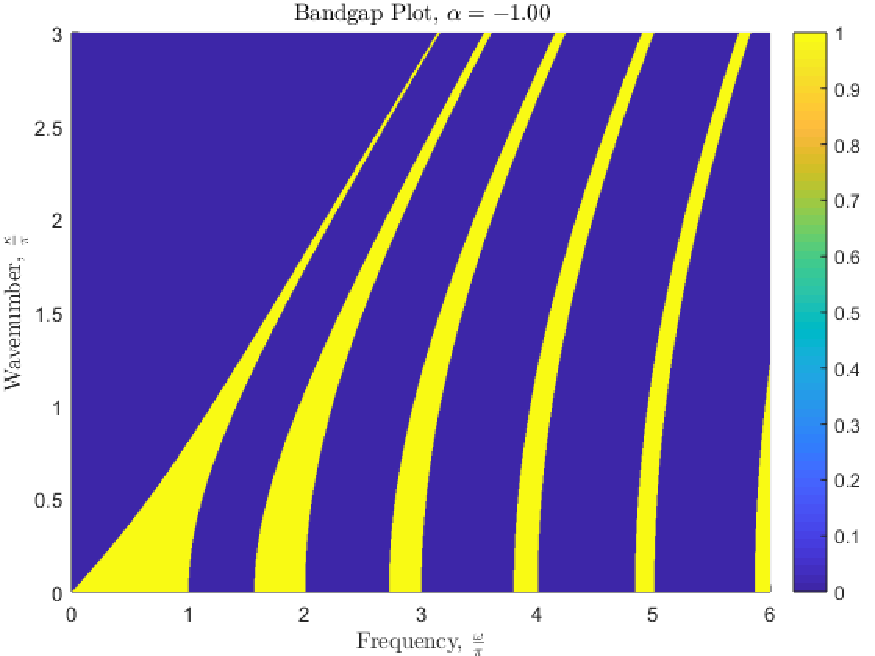
\includegraphics[scale=0.5]{TFR_Curls_BandgapPlot_alpha-1.pdf}
	\caption{\label{fig:TFR_Curls_BandgapPlot_alpha-1}}
\end{figure}

\section{Summary}
Chapter summary of the results and how they might be physically interpreted.
Speculate on future developments.